\section{Training} \label{sec:training}

The training stage precomputes and stores data to make the inference and evaluation stages faster and more efficient. Since all static and contextual embedding models in this thesis are pretrained, the term \emph{precomputation} stage is more accurate than \emph{training} stage. However, both terms will be used interchangeably to distinguish this phase from the subsequent inference phase.

This section provides details on the training stages for the Citation Recommender (\Cref{sec:citation-recommender}) and the Language Recommender (\Cref{sec:language-recommender}). The Hybrid Recommender, which merges data from both recommenders, is not part of the training stage. Instead, it integrates precomputed data from the Citation Recommender and the Language Recommender on-the-fly during inference (\Cref{sec:inference}).


\subsection{Citation Recommender} \label{sec:citation-recommender}

As elucidated in \Cref{sec:hybrid-recommender-architecture}, the Citation Recommender uses global document characteristics and citation-based features to generate recommendations.
\Cref{fig:citation-recommender} illustrates how the publication date, paper citation count, and author citation count are immediately provided by the base dataset, while the co-citation analysis and bibliographic coupling features are derived from the citations and references columns, respectively.

\begin{figure}[htb!]
    \centering
    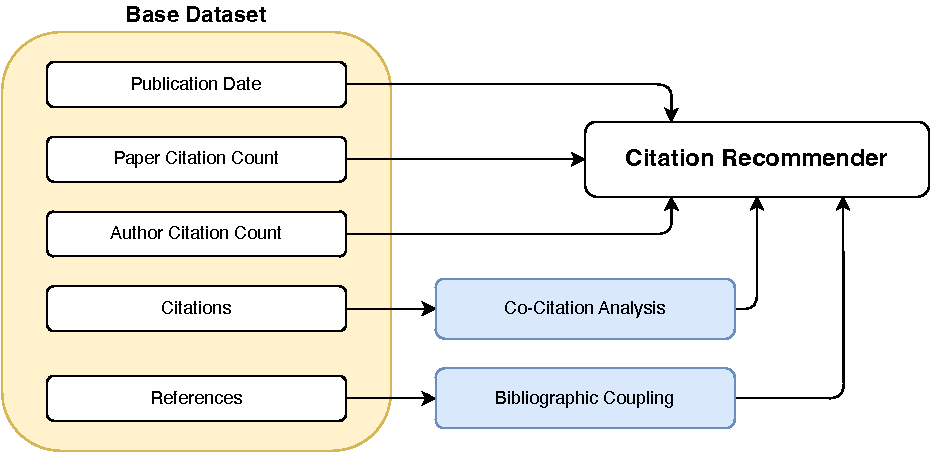
\includegraphics[width=0.9\textwidth]{diagrams/citation_recommender.pdf}
    \caption[Citation Recommender]{Inputs to the Citation Recommender. The publication date, paper citation count, and author citation count are immediately provided by the base dataset. The co-citation analysis and bibliographic coupling features are derived from the citations and references columns of the dataset, respectively.}
    \label{fig:citation-recommender}
\end{figure}

Given two papers from the \emph{readnext} dataset, the co-citation analysis score counts the number of shared citing papers in the citations column. Analogously, the bibliographic coupling score counts the number of shared cited papers in the references column. \Cref{fig:bibliographic_coupling_from_references} visualizes this process at the example of the bibliographic coupling score.

\begin{figure}[htb!]
    \centering
    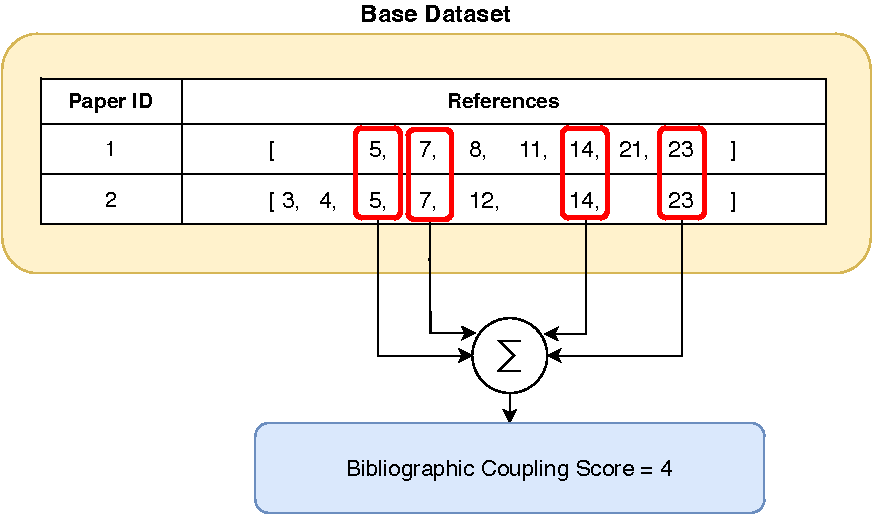
\includegraphics[width=0.7\textwidth]{diagrams/bibliographic_coupling_from_references.pdf}
    \caption[Bibliographic Coupling Score]{Computation of bibliographic coupling scores from the base dataset. The \emph{references} column contains four common items for the papers 1 and 2, resulting in a bibliographic coupling score of 4. For visualisation purposes, numeric paper IDs are utilized as identifiers in the figure, whereas unique Semantic Scholar URLs are used in the actual dataset.}
    \label{fig:bibliographic_coupling_from_references}
\end{figure}

During training, each document in the \emph{readnext} corpus is iteratively considered as the \emph{query paper}, with all remaining documents acting as \emph{candidate papers}. For each query paper, the pairwise co-citation analysis and bibliographic coupling scores with all candidate papers are computed and stored in a dataframe with corresponding document IDs.
Thus, time complexity during training grows quadratically with the corpus size.
For $n$ documents in the dataset, $n^2 - n$ pairwise scores are computed for each of the two features.

To circumvent quadratic growth for the memory and storage requirements, the Citation Recommender stores only the top 100 candidate papers with the highest co-citation analysis and bibliographic coupling scores for each query paper (see \Cref{sec:performance-considerations}).
Although not storing all pairwise scores to disk conserves memory, this approach does not decrease runtime since identifying the top 100 scores requires calculating all pairwise scores first.


\subsubsection*{Feature Weighting}

The Citation Recommender generates recommendations using a weighted average of the global document characteristics and citation-based features.
Therefore, not all features exert the same influence on the Citation Recommender. Instead, users can assign weights to each feature based on their preferences.
The weights are normalized to sum up to one, ensuring the results are not affected by the absolute magnitude of the weights.
Candidate papers with the best weighted average score are recommended to the user.

A caveat of this approach is that the raw feature values, such as the publication date (represented as a date) and the paper citation count (an integer), are not directly comparable.
To aggregate all five features into a single score, a rank-based method is used.


\subsubsection*{From Scores to Ranks}

The Citation Recommender first ranks all candidate papers according to each of the five features individually.
The ranking process assigns the top rank 1 to the most relevant candidate paper and increments the rank by 1 for each subsequent paper.
Candidate papers with more recent publication dates, higher citation counts, higher co-citation analysis and higher bibliographic coupling scores receive better rankings.
Ranks for global document characteristics remain constant across different query papers and must be computed only once.
In contrast, ranks for citation-based features are specific to each query paper and must be recomputed for each query paper.

The decision to store only the top 100 candidate papers for the co-citation analysis and bibliographic coupling scores prohibits the computation of exact ranks for all candidates beyond the top 100. Consequently, the ranks for the remaining candidates are uniformly set to 101, implying that there is no distinction between the 101st and all worse-ranked candidate papers.
Due to this nonlinearity, outliers in the positive direction with high scores have a stronger impact on the final recommendation ranking than outliers in the negative direction with low scores.
For consistency, the same ranking scheme is applied to the publication date, paper citation count, and author citation count features.


\subsubsection*{From Ranks to Points}

The final recommendation ranking could simply be calculated as the weighted average of the individual feature ranks, with lower average ranks leading to earlier recommendations. However, this method doesn't readily convey whether a particular weighted rank of e.g. $412$ is good or bad without knowing the specifics of the ranking system and the number of features involved.

For greater interpretability, the Citation Recommender translates feature ranks into \emph{points}, which are inversely related to the rank: the lower the rank, the higher the point score.
More precisely, the points are calculated as the difference between the maximum rank of $101$ and the actual feature rank, resulting in a range of $0$ to $100$ points.
These points are then weighted by the feature weights and summed to a weighted points score. Candidates with higher weighted points are considered more relevant and appear earlier in the final recommendation ranking.
The point-based system assigns zero contribution to candidate papers beyond the top $100$, which is more intuitive than a rank contribution of $101$.

The linear scaling of points from $0$ to $100$ in steps of $1$ is chosen to diminish the weighted score's dependence on individual features.
Superlinear scaling, like awarding $100$ points to the top-ranked candidate, $50$ to the next and $10$ to the third, excessively emphasizes outliers in a single feature.
For instance, a paper that is co-authored by Yoshua Bengio, the most-cited author in the dataset with a citation count of $372,099$, but ranks last in all other features might outperform a paper that ranks third across all features.
Hence, although the second paper is likely more relevant to the query paper, it would be recommended later than the first paper.


\subsection{Language Recommender} \label{sec:language-recommender}

In contrast to the Citation Recommender, the Language Recommender uses only a single column of the \emph{readnext} dataset: the paper abstracts. Its objective during training is to compute and store the similarity between any two abstracts in the corpus. To achieve this, the Language Recommender employs one of eight language models to embed each abstract into a vector space. Then, pairwise cosine similarities between all abstract embeddings are computed and stored.

Since each of the eight language models can be selected by the user during inference, embeddings and cosine similarities must be precomputed for all of them during the training stage.
As illustrated in \Cref{fig:language-recommender}, once the paper abstracts are tokenized, different language models do not interact with each other.
Therefore, embeddings and cosine similarities can be efficiently computed in parallel for all language models.

\begin{figure}[htb!]
    \centering
    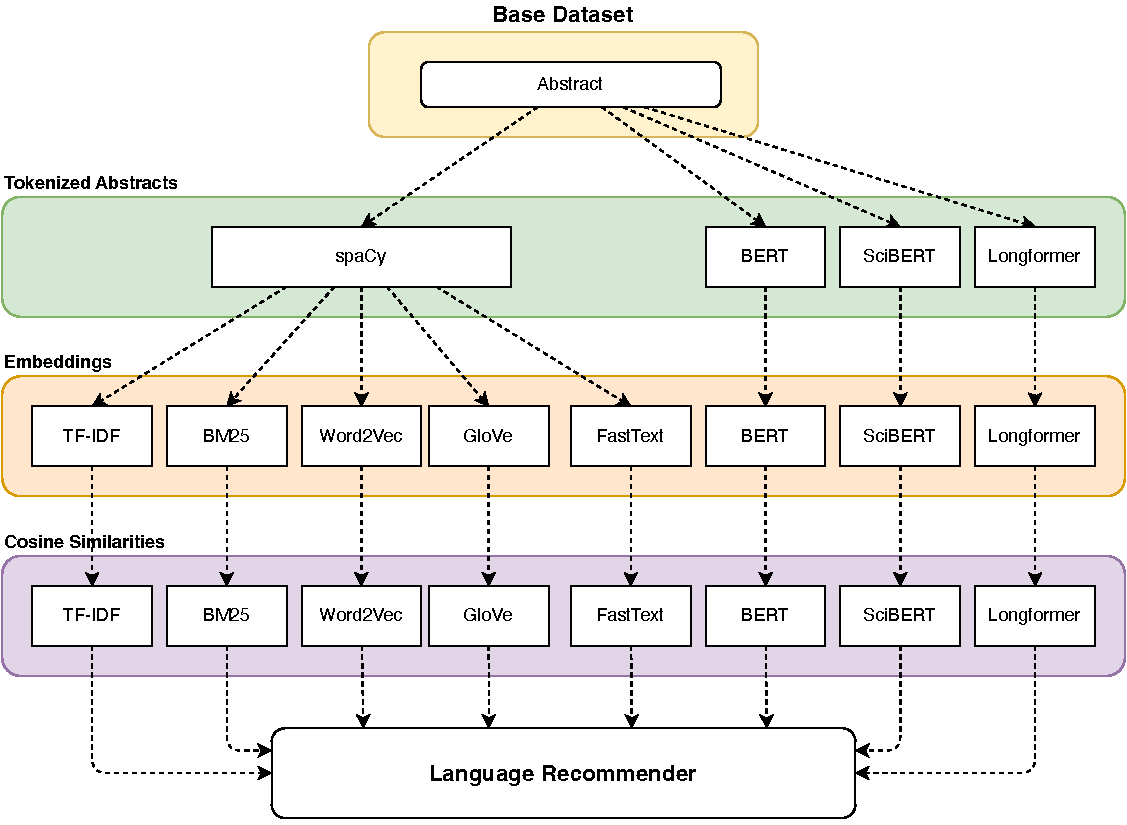
\includegraphics[width=\textwidth]{diagrams/language_recommender.pdf}
    \caption[Language Recommender]{Structure of the Language Recommender.
        First, the paper abstracts are tokenized. BERT, SciBERT and Longformer use a specialized tokenizer, while the remaining models use the \texttt{spaCy} \cite{HonnibalImprovedNonmonotonic2015} tokenizer. Then, each language model embeds the tokenized abstracts into a vector space. Finally, pairwise cosine similarities between all document embeddings are computed for all language models.}
    \label{fig:language-recommender}
\end{figure}

The cosine similarities are used to find abstracts most similar to a given query abstract.
For instance, when requested with the task to find the semantically most similar document to the paper \emph{Attention Is All You Need} by Vaswani et al. \cite{VaswaniAttentionAll2017} with BERT as the embedding model, the Language Recommender selects the data containing all precomputed BERT cosine similarities, filters it for the paper ID of \emph{Attention Is All You Need}, and returns the candidate paper with the highest cosine similarity.
Similar to the co-citation analysis and bibliographic coupling scores, only the top $100$ cosine similarities are stored for each query paper.

For the particular example above, $81$ out of $10,000$ papers have cosine similarities above $0.9$ with the paper \emph{Attention Is All You Need} as measured by BERT. The semantically most similar paper is \emph{Effective Approaches to Attention-based Neural Machine Translation} by Luong et al. \cite{LuongEffectiveApproaches2015} with a cosine similarity of $0.967$.
Using a different language model for the embedding step would result in a different ranking of the candidate papers.
The following sections describe the implementation and configuration of each language model in detail.


\subsubsection*{Keyword-based Models}

As explained in \Cref{sec:sparse-embeddings}, TF-IDF \cite{SaltonTermWeighting1987} and BM25 \cite{RobertsonOkapiTREC31995} are keyword-based models that generate sparse vector embeddings, where each embedding dimension corresponds to a single word in the vocabulary. The vocabulary consists of all unique words in the preprocessed text corpus, which in this case is the collection of all paper abstracts contained in the \emph{readnext} dataset.
The abstract embeddings are sparse vectors of the same length as the vocabulary, where each non-negative value represents the TF-IDF or BM25 score of the corresponding word in the abstract.


\subsubsection*{Tokenization and Preprocessing}

Before document embeddings can be computed, the raw abstracts must be tokenized and preprocessed. In case of TF-IDF and BM25, the tokenization process is performed by the \texttt{spaCy} \cite{HonnibalImprovedNonmonotonic2015} library, more specifically by the pretrained \texttt{en\_core\_web\_sm} model \footnote{\url{https://spacy.io/models/en\#en\_core\_web\_sm}} that is able to tokenize and preprocess English text. \texttt{spaCy} splits the text into a list of individual tokens and collects metadata about each token, such as its part-of-speech tag, its lemma, and whether it is a stop word. This information can be used for further text processing steps.

The preprocessing steps by \texttt{spaCy} for the TF-IDF and BM25 models include:

\begin{itemize}
    \item Converting all tokens to lowercase.
    \item Lemmatizing all tokens. Lemmatization helps to reduce the vocabulary size by reducing a word to its base form, e.g. \emph{running} to \emph{run}.
    \item Removing non-alphanumeric characters, non-ASCII characters, punctuation, digits, and whitespace.
    \item Removing stop words.
          Stop words are words that occur frequently in the English language and are thus considered uninformative for any particular document. Examples of stop words are \emph{the}, \emph{a}, and \emph{is}.
          The \texttt{spaCy} library uses a predefined list of $326$ English stop words that do not contribute to the document embeddings.
\end{itemize}

\Cref{fig:spacy} illustrates the tokenization and preprocessing process of \texttt{spaCy} on a practical example.
Post tokenization, the tokens can be passed to the TF-IDF and BM25 models to compute abstract embeddings.

\begin{figure}[htb!]
    \centering
    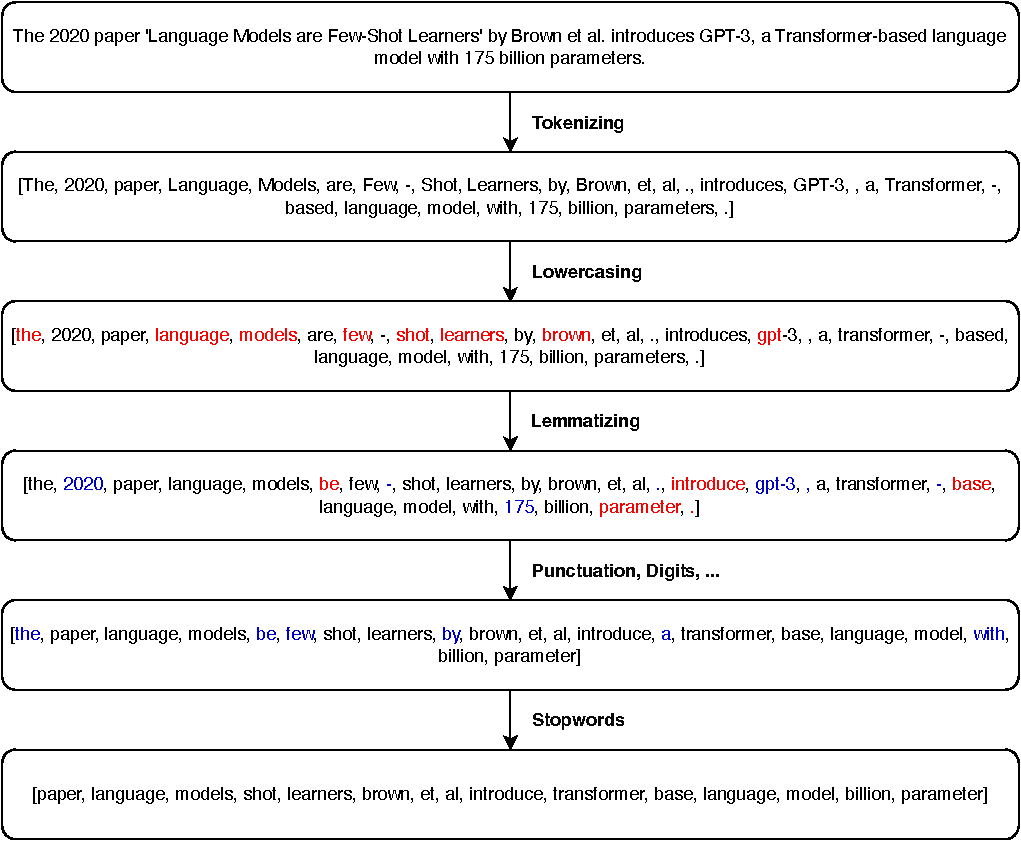
\includegraphics[width=\textwidth]{diagrams/spacy.pdf}
    \caption[Tokenization and Preprocessing]{Tokenization and text preprocessing with \texttt{spaCy}. Red indicates tokens that were modified from the previous step, while blue indicates tokens that are removed in the next step. First, the input sentence is tokenized into a list of individual tokens. Each token is then lowercased, lemmatized, and stripped of non-alphanumeric characters, punctuation, digits, and whitespace. Finally, stop words are removed. The preprocessed tokens are used by language models to compute document embeddings.
    }
    \label{fig:spacy}
\end{figure}


\subsubsection*{TF-IDF}

The TF-IDF model is implemented with the \texttt{scikit-learn} library \cite{PedregosaScikitlearnMachine2011} according to \Cref{eq:tf-sklearn} for the term frequency and \Cref{eq:idf-sklearn} for the inverse document frequency.
The TF-IDF values for all abstract tokens are computed and stored in a sparse matrix of dimension $|D| \times |V|$, where $|D| = 10,000$ is the number of documents in the training corpus and $|V|=21,240$ is the size of the vocabulary.
In practice, specialized storage formats for sparse matrices are used to reduce memory consumption.

Each row of the matrix represents the TF-IDF document embedding of a single abstract.
To keep the connection to the corresponding paper, the embeddings are stored together with their document IDs in a dataframe.
Based on this representation, the semantic similarity between any two abstracts can be computed by looking up the corresponding rows in the dataframe by their IDs and calculating the cosine similarity between their embeddings.


\subsubsection*{BM25}

The BM25 model is implemented in its BM25+ variant with \Cref{eq:bm25+-tf} for the term frequency and \Cref{eq:bm25-idf} for the inverse document frequency.
The free parameters are set to $k_1 = 1.5$, $b = 0.75$, and $\delta = 1$ as implemented in the \texttt{rank\_bm25} Python library \cite{BrownRankBM25Collection2020}.

The vocabulary size and thus the dimensions of the BM25 document embeddings are identical to the dimensions of the TF-IDF document embeddings since the vocabulary is determined by the underlying text corpus and not by any of the two models. Similarly, the cosine similarities are computed in the same fashion as for the TF-IDF model.


\subsubsection*{Static Embedding Models}

Static embedding models, such as Word2Vec \cite{MikolovEfficientEstimation2013}, FastText \cite{BojanowskiEnrichingWord2017}, and GloVe \cite{PenningtonGloveGlobal2014}, generate fixed-length dense vector embeddings for each word in the vocabulary.
As for the keyword-based models, tokenization is performed by the \texttt{spaCy} library with the same preprocessing pipeline.
The processed tokens are subsequently passed to each of the three static embedding models to compute document embeddings for all abstracts in corpus. Within \emph{readnext}, Word2Vec, FastText, and GloVe are implemented via their \texttt{gensim} interface \cite{RehurekGensimPython2011} using pretrained models

Token embeddings within the same document are averaged to compute document embeddings. As before, document embeddings are stored together with their corresponding document IDs in a dataframe. Document similarities are again computed as the cosine similarity between any pair of document embeddings.

\paragraph{Word2Vec}

For Word2Vec, we implemented the \emph{word2vec-google-news-300} model. This model is pretrained on the Google News Corpus \cite{MikolovEfficientEstimation2013} with approximately $100$ billion words. The embedding dimension is set to $300$.
The model is, again provided by the from the \emph{gensim-data} GitHub repository\footnote{\url{https://github.com/RaRe-Technologies/gensim-data}}. The file size of the downloaded model is $3.64$ GB.

\paragraph{FastText}

We used the FastText model from Grave et al. \cite{GraveLearningWord2018}, pretrained on English Wikipedia and the Common Crawl corpus. As for Word2Vec, the embedding dimension is set to $300$. Specific to the FastText model, the character $n$-gram length is set to $5$.
The pretrained model can be downloaded from the FastText website\footnote{\url{https://fasttext.cc/docs/en/crawl-vectors.html\#models}}. The size of the downloaded model is $7.24$ GB.

\paragraph{GloVe}

For GloVe, we opted for the \emph{glove.6B.300d} model, pretrained on Wikipedia 2014 and Gigaword 5 \cite{PenningtonGloveGlobal2014} with around $6$ billion tokens and a vocabulary size of $400,000$. The embedding dimension is again set to $300$. The pretrained word embeddings can be downloaded from the Stanford NLP website\footnote{\url{https://nlp.stanford.edu/projects/glove/}}. The size of the downloaded embeddings is $1.04$ GB.


\subsubsection*{Contextual Embedding Models}

Models such as BERT \cite{DevlinBERTPretraining2019}, SciBERT \cite{BeltagySciBERTPretrained2019}, and Longformer \cite{BeltagyLongformerLongDocument2020} are contextual embedding models that produce dense vector representations of fixed length for each token in the input text. The distinctive characteristic of these representations is their contextual nature: the vector representation of a token is influenced by the surrounding context in which the token appears.
Thus, unlike static embedding models that map each word to a single embedding vector, contextual embedding models generate different vector representations for polysemous words depending on their meaning in the given context.

Since BERT, SciBERT and Longformer are all based on the Transformer architecture \cite{VaswaniAttentionAll2017}, they are referred to as \emph{Transformer models} in the following.

\subsubsection*{Tokenization for Transformer Models}

Within \emph{readnext}, Transformer models are implemented using the open-source \texttt{transformers} library \cite{WolfHuggingFaceTransformers2020}. This library provides a unified interface to numerous pretrained \ac{LLMs}.
\texttt{transformers} is actively developed and maintained by Hugging Face\footnote{\url{https://huggingface.co/}}.

In contrast to keyword-based and static embedding models that use \texttt{spaCy} for tokenization, the text preprocessing steps for Transformer models are tailored to each model individually, as it is crucial that the input format during inference matches the one used during pretraining.
Whereas \texttt{spaCy} produces \emph{text} tokens, Transformer tokenizers generate integer token \emph{IDs} that correspond to the indices of the tokens in the pretrained model's vocabulary.
The subsequent paragraphs delineate the tokenization process for each Transformer model in detail.


\subsubsection*{BERT}

We employed the \emph{bert-base-uncased} version of BERT pretrained on the BooksCorpus (800 million words) and English Wikipedia (2,500 million words). The \emph{bert-base-uncased} model can be accessed via the Hugging Face Model Hub\footnote{\url{https://huggingface.co/bert-base-uncased}}.

BERT employs the \emph{WordPiece} tokenizer \cite{WuGoogleNeural2016}, a subword tokenization method that initially tokenizes at whitespace and punctuation. If the resultant tokens are not found in the model's vocabulary, they are further split into smaller subwords until all word pieces belong to the vocabulary. Subwords are prefixed with \texttt{\#\#} to distinguish them from regular words. The vocabulary of the \emph{bert-base-uncased} model comprises roughly $30,000$ tokens \cite{DevlinBERTPretraining2019}.

In BERT's input representation, special tokens play a pivotal role. The \texttt{[CLS]} token starts each input sequence and acts as a collective representation for classification tasks. The \texttt{[SEP]} token separates different sentences or sequence pairs. For single-sequence tasks, it is attached at the end of the sequence, while for two-sequence tasks, it is added at the end of both sequences. The \texttt{[PAD]} tokens are utilized to pad shorter sequences to a common length, and \texttt{[UNK]} tokens represent words not found in the vocabulary after WordPiece tokenization. The \texttt{[MASK]} tokens are used for the masked language model objective during pretraining \cite{DevlinBERTPretraining2019}.

The maximum input length for BERT is $512$ tokens, inclusive of the special tokens. This limitation becomes critical in the context of this thesis, as some paper abstracts in the training corpus exceed this limit. Beltagy et al. \cite{BeltagyLongformerLongDocument2020} elucidate common workarounds to manage this issue. The simplest strategy is to truncate all abstracts to a maximum length of $512$ tokens \cite{XieUnsupervisedData2020}. However, this strategy might discard potentially relevant information. An alternative strategy is to divide the abstracts into smaller sequences with maximum length of $512$ tokens, processing each sequence separately, and combining the resulting sequence embeddings \cite{JoshiBERTCoreference2019}. Although this strategy retains all information, it is computationally expensive.

Given that only $0.58$\% of all abstracts in the \emph{readnext} corpus exceed the maximum sequence length of $512$ tokens, we decided to truncate longer abstracts to this maximum length. Conversely, shorter abstracts are padded with \texttt{[PAD]} tokens to a length of $512$ tokens to ensure that all tokenized abstracts are of the same length.

BERT generates token embeddings of dimension $768$. The document embedding for the entire abstract is computed as the mean of all token embeddings within the abstract. The resulting document embeddings are stored alongside their corresponding document ID in a dataframe from which the pairwise cosine similarities can be computed.


\subsubsection*{SciBERT}

For SciBERT, we selected the \emph{scibert\_scivocab\_uncased} version, accessible via the Hugging Face Model Hub\footnote{\url{https://huggingface.co/allenai/scibert\_scivocab\_uncased}}.
While SciBERT and BERT share the same architecture, they differ in their pretraining corpus and vocabulary.
SciBERT is pretrained on a large corpus of scientific text consisting of 1.14 million papers from the Semantic Scholar corpus (amounting to 3.17 billion tokens) \cite{BeltagySciBERTPretrained2019}. The corpus is composed of papers from a variety of scientific disciplines, including Computer Science, Physics, and Biomedicine.

Consequently, SciBERT's vocabulary is tailored to scientific text and includes a significant number of scientific terms that are not part of BERT's vocabulary. Therefore, scientific terms that would be tokenized into multiple subwords or even into \texttt{[UNK]} tokens by BERT's tokenizer can often be tokenized into a single subword by SciBERT's tokenizer, resulting in a more accurate representation of the input text. The vocabulary size of the \emph{scibert\_scivocab\_uncased} model is set to $30,000$ tokens to align with the vocabulary size of the \emph{bert-base-uncased} model \cite{BeltagySciBERTPretrained2019}.

The tokenization process and the special tokens in SciBERT are identical to those in BERT. SciBERT also uses WordPiece tokenization, adds the same special tokens to the input sequence, has the same maximum sequence length of $512$ tokens, and generates token embeddings of dimension $768$. The document embedding computation is also identical to BERT: the document embedding is computed as the mean of all token embeddings within the abstract.


\subsubsection*{Longformer}

We opted for the \emph{longformer-base-4096} version of the Longformer model, again provided by the Hugging Face Model Hub\footnote{\url{https://huggingface.co/allenai/longformer-base-4096}}.
Whereas BERT is pretrained with \ac{MLM} and \ac{NSP} tasks, Longformer relies solely on the \ac{MLM} task.
Unlike BERT, Longformer's pretraining does not start from scratch; instead, it uses the weights of the RoBERTa model \cite{LiuRoBERTaRobustly2019} as initialization.
The Longformer model is pretrained on a compiled corpus of long documents comprising subsets of the BooksCorpus \cite{ZhuAligningBooks2015}, the English Wikipedia, the Realnews dataset \cite{ZellersDefendingNeural2019} and the Stories corpus \cite{TrinhSimpleMethod2019}.

While the BERT tokenizer truncates input sequences to a maximum length of $512$ tokens, the Longformer tokenizer can handle input sequences of up to $4,096$ tokens due to its sliding window attention mechanism described in \Cref{sec:contextual-embeddings}.
By default, Longformer's sliding window attention mechanism uses a size of $512$ tokens.
As none of the abstracts in the \emph{readnext} corpus exceed a length of $4,096$ tokens, truncation is not required for the Longformer model. Similar to BERT, all abstracts are padded with special \texttt{<pad>} tokens to a common length of $4,096$ tokens.

The principal methodological difference to BERT's tokenizer is that Longformer's tokenizer uses Byte-Pair Encoding (BPE) \cite{SennrichNeuralMachine2016} instead of WordPiece tokenization \cite{WuGoogleNeural2016}. Consequently, the Longformer tokenizer employs a different set of special tokens. The start and end tokens are \texttt{<s>} and \texttt{</s>}, respectively. Unlike the BERT tokenizer, which uses \texttt{\#\#} to indicate subwords, the Longformer tokenizer adds the special token \texttt{Ġ} to represent spaces. In Longformer, subwords are distinguished from regular words by not being prefixed with a space token.

\begin{table}[htb!]
    \centering
    \begin{tabular}{l p{5cm} p{5cm}}
        \toprule
        \textbf{Feature}       & \textbf{BERT}          & \textbf{Longformer}                                        \\
        \midrule
        \# Parameters          & 110M (BERT-base)       & 125M (RoBERTa-base)                                        \\
        Embedding Dimension    & 768                    & 768                                                        \\
        Max. Sequence Length   & 512                    & 4096                                                       \\
        Training Data          & BooksCorpus, Wikipedia & Long Documents (BooksCorpus, Wikipedia, Realnews, Stories) \\
        Training Task          & MLM \& NSP             & MLM                                                        \\
        Weight Initialization  &                        & RoBERTa                                                    \\
        Attention Mechanism    & Full Self-Attention    & Sliding Window Attention                                   \\
        Attention Window Size  & 512                    & 512                                                        \\
        Tokenization Algorithm & WordPiece              & Byte-Pair Encoding                                         \\
        Start Token            & \texttt{[CLS]}         & \texttt{<s>}                                               \\
        End Token              & \texttt{[SEP]}         & \texttt{</s>}                                              \\
        Pad Token              & \texttt{[PAD]}         & \texttt{<pad>}                                             \\
        Subword Prefix         & \texttt{\#\#}          &                                                            \\
        Space Token            &                        & \texttt{Ġ}                                                 \\
        \bottomrule
    \end{tabular}
    \caption[BERT vs. Longformer]{Model properties of BERT and Longformer.
        Longformer initializes its weights from the RoBERTa model encompassing $125$ million parameters compared to $110$ million parameters for BERT-base. The Longformer tokenizer uses Byte-Pair Encoding instead of WordPiece tokenization and a different set of special tokens. The most significant difference between the two models is that Longformer uses a sliding window attention mechanism instead of full self-attention to better process long documents. Accordingly, Longformer is pretrained on a corpus of exclusively long documents and can handle input sequences of up to $4,096$ tokens.
    }
    \label{tab:bert_longformer_tokenizer}
\end{table}

\begin{figure}[htb!]
    \centering
    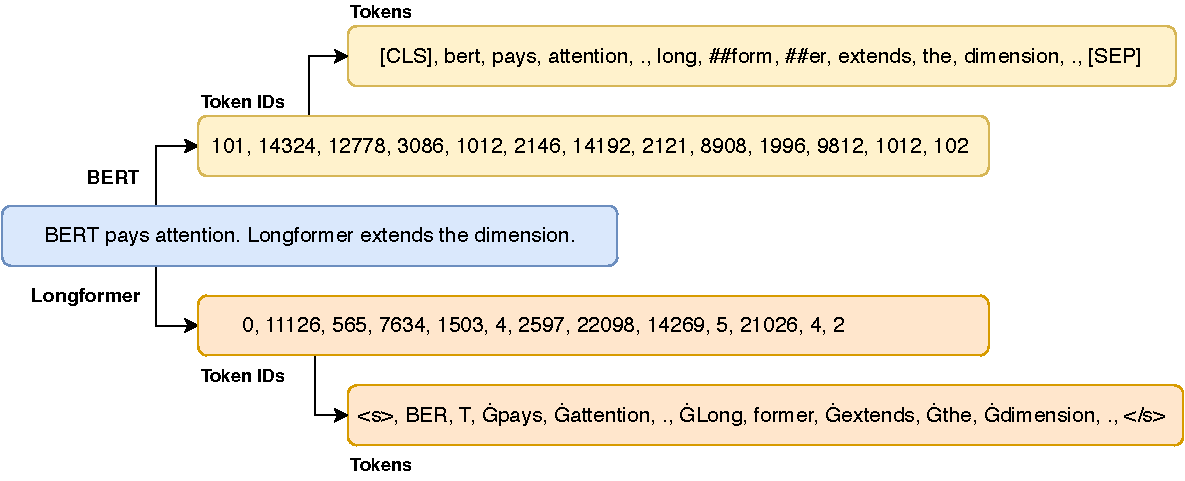
\includegraphics[width=\textwidth]{diagrams/bert_longformer_tokenizer.pdf}
    \caption[BERT vs. Longformer Tokenization]{Tokenization example for BERT and Longformer. Both tokenizers produce token IDs rather than text tokens.
        Each token ID corresponds to a unique word piece in the vocabulary. BERT uses the \texttt{\#\#} symbol to indicate subwords, whereas Longformer uses the \texttt{Ġ} symbol for whitespace.}
    \label{fig:bert_longformer_tokenizer}
\end{figure}

\Cref{tab:bert_longformer_tokenizer} illustrates the conceptual differences between BERT and Longformer, whereas \Cref{fig:bert_longformer_tokenizer} compares their tokenization processes on the example sentence pair \emph{BERT pays attention. Longformer extends the dimension.} Note that, unlike traditional tokenization approaches, Transformer models do not remove punctuation from the input text. Instead, punctuation is treated as a separate token.

Like BERT and SciBERT, Longformer aggregates token embeddings into document embeddings by averaging all token embeddings within the abstract. Cosine similarities between document embeddings are computed in the same manner as for previous models.
